% !TEX program = pdflatex
\documentclass[11pt,a4paper]{article}

\usepackage[utf8]{inputenc}
\usepackage[T1]{fontenc}
\usepackage{lmodern}
\usepackage{geometry}
\geometry{margin=1in}
\usepackage{amsmath,amssymb}
\usepackage{siunitx}
\usepackage{graphicx}
\usepackage[font=small,labelfont=bf,labelsep=endash]{caption}
\usepackage{booktabs}
\usepackage{physics}
\usepackage{cite}
\usepackage{hyperref}
\usepackage{float}
\hypersetup{colorlinks=true,linkcolor=blue,citecolor=blue,urlcolor=blue}

\title{Design Methodology for a Dual-Jet Hovering Disc with Concentric Air Curtains:\\
Model, Non-Dimensionalization, and Physical Assumptions}
\author{ }
\date{ }

\begin{document}

\maketitle

\begin{abstract}
This paper presents a design-oriented physical model for a hovering disc sustained by two concentric air jets:
an outer annular jet that forms an aerodynamic curtain to confine the inner flow and an inner jet that maintains the central cushion pressure.
The analysis uses a low-Mach compressible, axisymmetric core model with an anisotropic Stokes--Darcy closure to approximate the pressure and velocity fields in the cushion region.
A detailed discussion of the model's assumptions and their physical validity is provided, along with a complete nomenclature of symbols used throughout the work.
\end{abstract}

\begin{figure}[t]
  \centering
  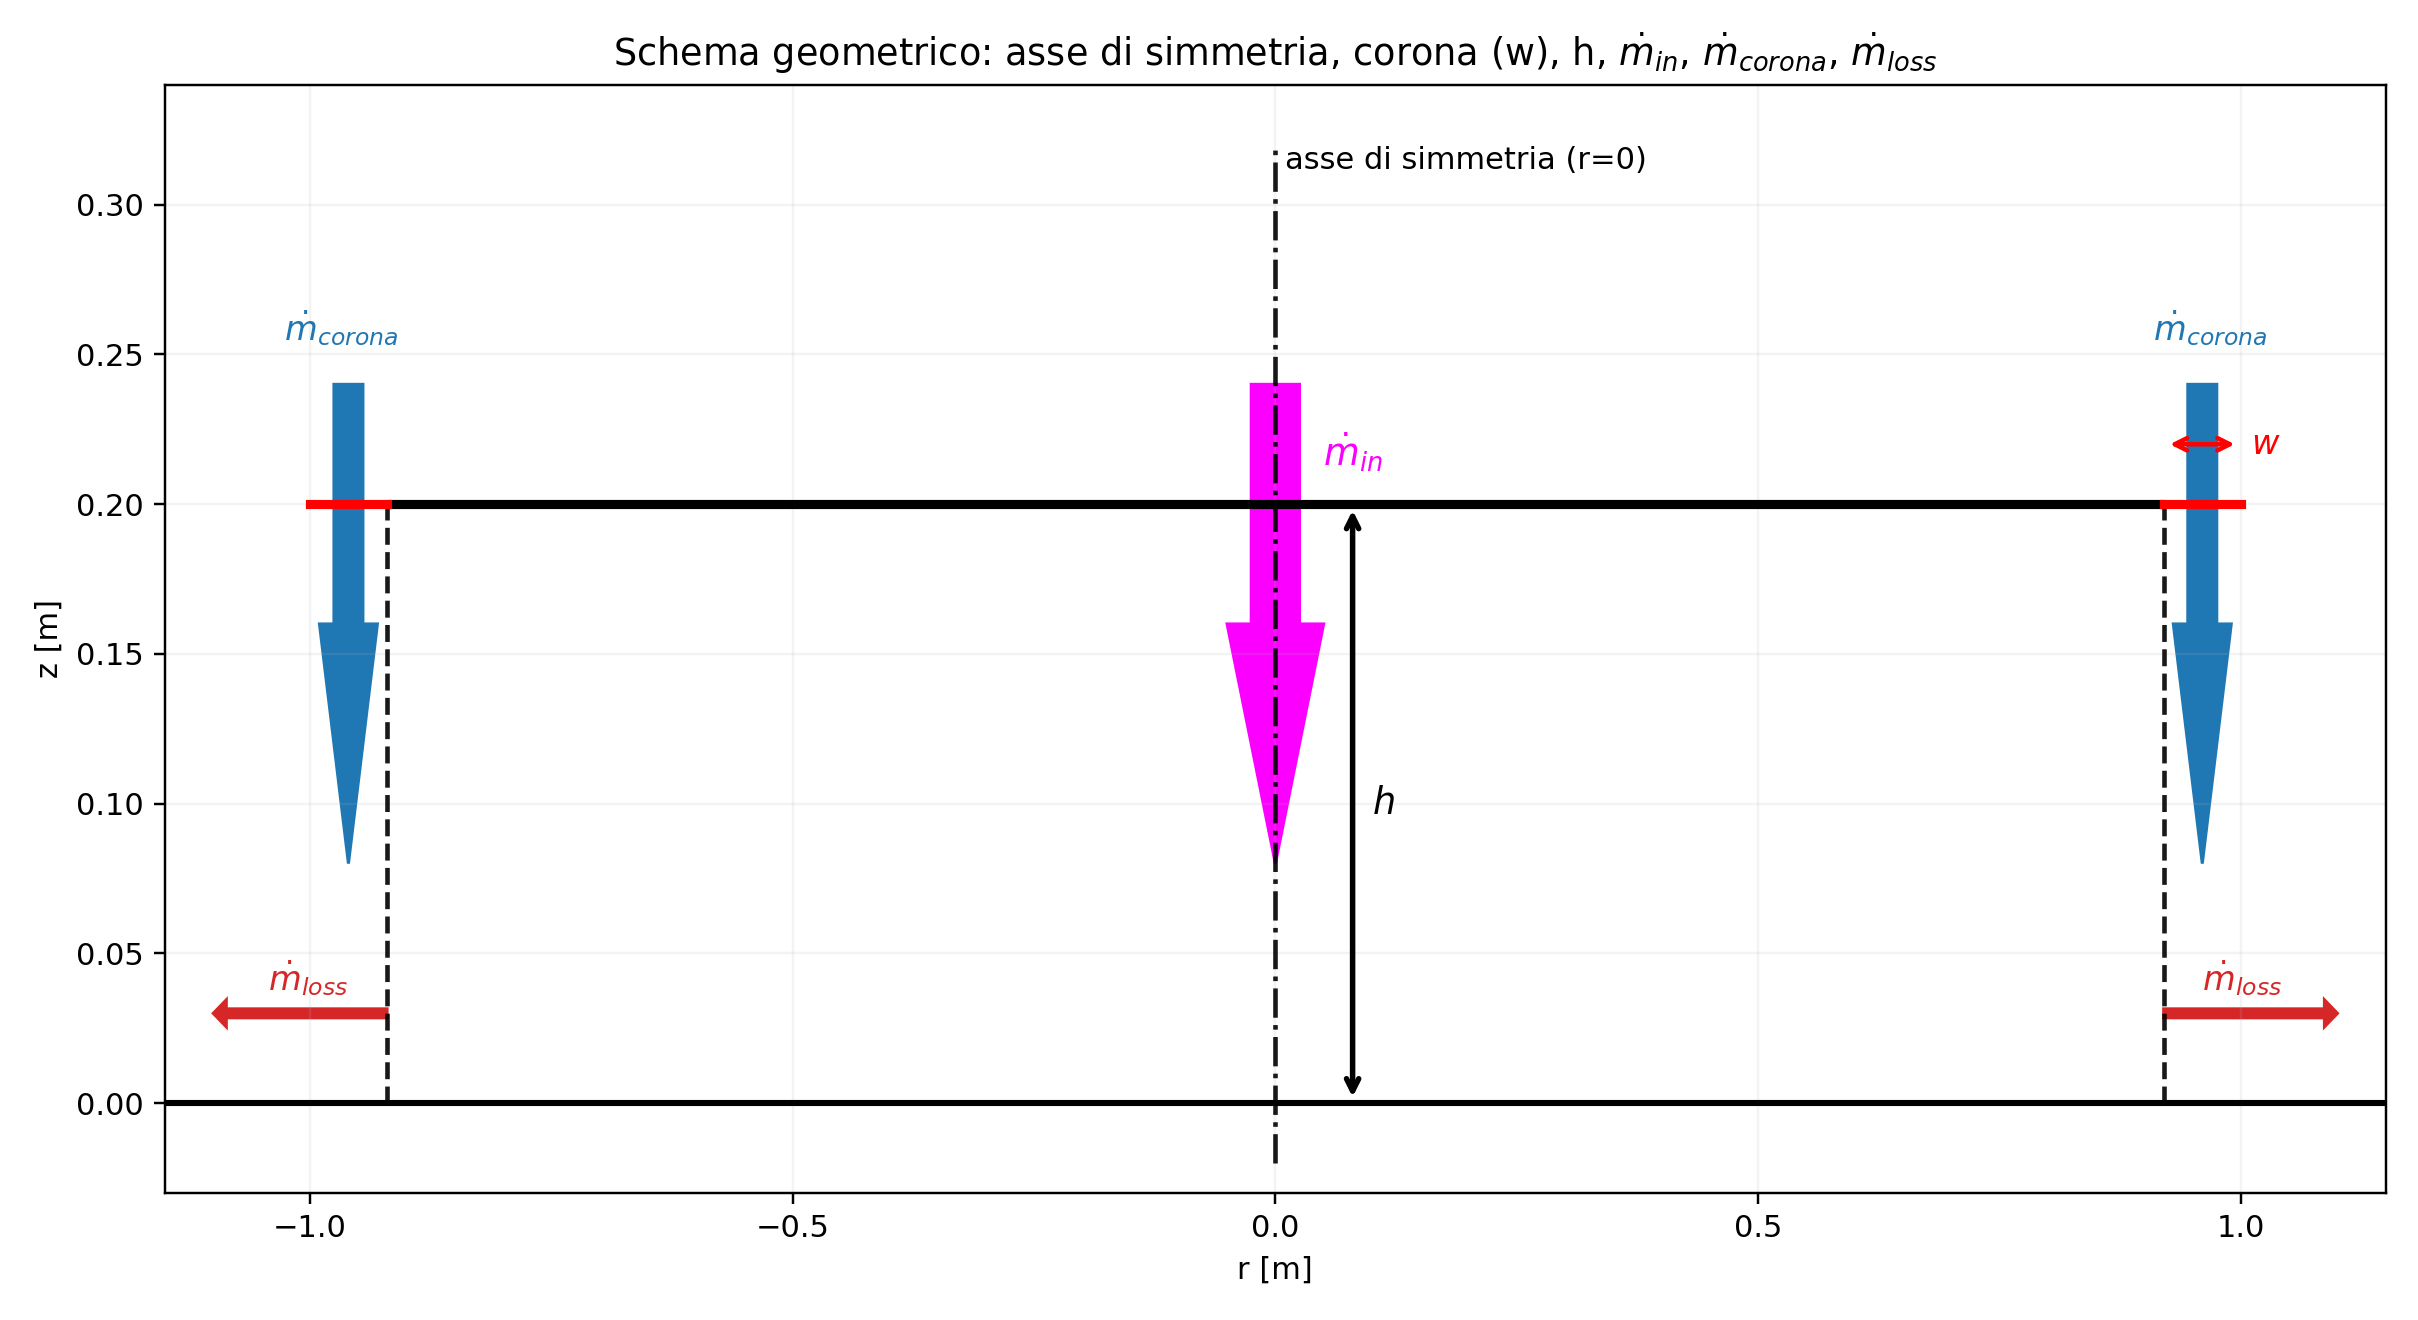
\includegraphics[width=0.95\linewidth]{../figs/schema_geometry.png}
  \caption{Schematic of the hovering disc with two concentric jets: the outer annular curtain and the central make-up flow.}
  \label{fig:geometry}
\end{figure}

\section{Geometry and Notation}
\label{sec:geometry}
The geometry follows Fig.~\ref{fig:geometry}, defining the coordinate system and characteristic dimensions:
\begin{itemize}
  \item $R_{\mathrm{tot}}$ -- total radius of the disc.
  \item $h$ -- hovering height from the ground.
  \item $w$ -- width of the peripheral leakage ring; $R^{-}=R_{\mathrm{tot}}-w$ is its inner radius.
  \item $b$ -- thickness of the outer annular jet slot.
  \item $h_{\mathrm{eff}}$ -- effective sealing height (characteristic of curtain recirculation).
  \item $p_0$ -- ambient pressure; $p_c=W/(\pi R_{\mathrm{tot}}^2)$ -- cushion pressure supporting the load $W$.
  \item $U_{\mathrm{out}}$, $\rho_j$ -- speed and density of the outer jet.
  \item $\mu$ -- dynamic viscosity; $R_g$ -- specific gas constant for air.
  \item $\dot{m}_{\mathrm{in}}$ -- air mass flow entering internal region.
  \item $\dot{m}_{\mathrm{out}}$ -- air mass flow of outer region.
  \item $\dot{m}_{\mathrm{loss}}$ -- air mass flow exiting internal region.
  \item $b_0$ -- slot thickness of the outer curtain jet at injection.
  \item $H$ -- effective curtain height (equal to $h$ in this study, representing the vertical extent over which the curtain resists leakage).
\end{itemize}

\section{Model Overview}
\label{sec:model-overview}

The cushion region ($0\le r\le R^{-},\ 0\le z\le h$) is filled with air at variable pressure, temperature, and density.
The mean flow satisfies an anisotropic Stokes--Darcy closure:
\begin{equation}
  u = -\frac{\kappa_r}{\mu}\,\partial_r p,\qquad
  w = -\frac{\kappa_z}{\mu}\,\partial_z p,
\end{equation}
with permeability coefficients $\kappa_r=\alpha_r h^2$ and $\kappa_z=\alpha_z h^2$, where $\alpha_r$ and $\alpha_z$ are empirical dimensionless parameters encoding the overall resistance of the confined air layer.

The continuity and state relations read
\begin{equation}
  \frac{1}{r}\,\partial_r\!\left(r\rho u\right)+\partial_z(\rho w)=0,\qquad
  p=\rho R_g T.
\end{equation}
Elimination of $u,w$ gives the pressure formulation:
\begin{equation}
  \frac{1}{r}\partial_r(r\rho\kappa_r\partial_r p)+\partial_z(\rho\kappa_z\partial_z p)=0.
\end{equation}




\section{Simulation Methodology}
\label{sec:simulation-method}

The numerical procedure has been redeveloped to consistently include the coupled dynamics between the cushion core and the surrounding outer jet, explicitly accounting for the mechanisms of jet impingement, wall-jet transition, and the formation of the sealing flow beneath the disc. The aim of this new framework is to determine the steady velocity and pressure fields in both the inner and outer flow regions by enforcing a mutual equilibrium condition between the overpressurized core and the outer annular jet.

\subsection*{1. Physical description and domain coupling}

The hover system can be decomposed into two interconnected flow regions:
\begin{itemize}
    \item The \textit{core cavity} ($0 \le r \le R^-,\, 0 \le z \le h$), filled with quasi-stagnant, pressurized air that supports the load and reacts to leakage and entrainment;
    \item The \textit{outer-jet region}, comprising the annular curtain of high-velocity air expelled through the peripheral slot at $r = R^-$, its impingement on the ground surface, and its subsequent radial transition into a wall jet.
\end{itemize}

The outer jet issues downward from the slot and impinges on the ground, creating a stagnation region and a local overpressure near the disk rim. The jet then deflects radially outward, forming a thin wall jet that develops along the ground surface. The combination of the impinging flow and the near-ground shear layer generates a local pressure barrier that inhibits radial leakage of the core air — this is the so-called \textit{seal effect}. The seal arises from the balance between the momentum of the impinging jet and the static pressure beneath the disc. Its strength depends on the slot exit velocity, the hover gap $h$, and the radial expansion geometry of the outer curtain. As the hover height increases, the jet impingement weakens, reducing the seal efficiency and leading to greater leakage; conversely, a smaller hover gap intensifies the impingement and raises the rim pressure, enhancing the sealing action.

The two regions interact strongly: the core overpressure modifies the effective slot exit conditions and, therefore, the outer-jet momentum and impingement behavior. In turn, the outer-jet impingement and wall-jet transition determine the pressure boundary condition acting on the core rim. The equilibrium between these coupled mechanisms defines the stationary state of the hover system.

\subsection*{2. Governing equations and coupling formulation}

In the core region, the flow is represented by a quasi-laminar Darcy–Stokes formulation:
\begin{equation}
u = -\frac{\kappa_r}{\mu}\,\partial_r p, 
\qquad
w = -\frac{\kappa_z}{\mu}\,\partial_z p,
\end{equation}
\begin{equation}
\frac{1}{r}\partial_r\left(r\,\rho\,\kappa_r\,\partial_r p\right)
+ \partial_z\left(\rho\,\kappa_z\,\partial_z p\right) = 0,
\quad p = \rho R_g T.
\end{equation}

Boundary conditions are:
\begin{itemize}
  \item Symmetry at the centerline ($r = 0$);
  \item No-normal-flow at the upper and lower boundaries ($z = 0$ and $z = h$);
  \item A rim-pressure boundary at $r = R^-$, determined dynamically from the outer-jet solution.
\end{itemize}

The outer jet is represented by a reduced-order model that captures its impingement dynamics and wall-jet evolution. The impingement pressure distribution $p_\text{imp}(r,z)$ and the resulting wall-jet pressure decay are expressed through a non-dimensional profile function $\Phi(\zeta)$:
\begin{equation}
p_\text{rim}(z) = p_0 + \rho_j U_{\text{out}}^2 \Phi(\zeta),
\qquad \zeta = \frac{z}{H},
\end{equation}
where $\Phi(\zeta)$ describes the normalized pressure field through the impingement and near-wall zones, obtained from empirical or semi-analytical jet correlations. The model also computes entrainment and radial mass transport along the ground, linking the jet’s kinetic energy to the sealing pressure beneath the rim.

\subsection*{3. Iterative coupling and stationary equilibrium}

The numerical algorithm follows a coupled iterative procedure:
\begin{enumerate}
    \item Initialize an estimate for the outer-jet exit velocity $U_{\text{out}}$ and flow rate $\dot{m}_{\text{out}}$, together with geometric parameters of the slot and hover gap.
    \item Solve the outer-jet model to determine the impingement pressure distribution $p_\text{rim}(z)$, the local stagnation overpressure, and the entrainment rates associated with the wall-jet transition.
    \item Apply $p_\text{rim}(z)$ as the boundary condition at $r = R^-$ and solve the governing equations for the core region to obtain the pressure field $p(r,z)$ and velocity components $(u,w)$.
    \item Compute the average cushion pressure $\overline{p}_{\text{core}}$ and the corresponding load-carrying capacity. Compare it to the target load or hover condition.
    \item If the difference exceeds the convergence tolerance, update $U_{\text{out}}$ (and consequently $p_\text{rim}$) according to the deviation between the core and target pressures, then repeat from step~2.
    \item Convergence is achieved when the core and outer-jet fields reach mutual equilibrium, such that the mass fluxes and rim pressures are self-consistent.
\end{enumerate}

At convergence, the model ensures:
\begin{equation}
\dot{m}_\text{in} = \dot{m}_\text{leak} + \dot{m}_\text{out},
\end{equation}
and the pressure and velocity fields satisfy both global mass conservation and local momentum balance across the core–jet interface. The resulting steady configuration reproduces the observed \textit{seal equilibrium}, where the outer jet dynamically maintains the overpressure within the core while being itself modulated by it.

\subsection*{4. Outputs and physical interpretation}

Once equilibrium is achieved, the simulation provides:
\begin{itemize}
  \item The complete pressure and velocity fields $(p,\,u,\,w)$ in the core cavity;
  \item The rim pressure and wall-jet profiles in the outer region;
  \item Mass flow rates and entrainment coefficients for both zones;
  \item The effective lift capacity and power requirement of the hover system;
  \item Sensitivity of the equilibrium height and seal efficiency to slot geometry, supply flow, and ambient pressure.
\end{itemize}

The improved numerical scheme thus integrates the physical phenomena of outer-jet impingement, wall-jet transition, and sealing behavior directly into the steady-state solution. By enforcing the mutual consistency of the core and jet regions, it provides a more realistic and predictive model of the hover-disc equilibrium than the previous decoupled approach.



\section{Validity of Modeling Assumptions}
\label{sec:validity-of-modeling-assumptions}

\subsection{Low-Mach Compressibility}
The jets have typical velocities $U_{\mathrm{out}}\approx30$--$60\,$m/s, leading to a Mach number $Ma=U/a\approx0.1$--$0.2$ with $a\simeq343\,$m/s.
This regime justifies a \emph{low-Mach} formulation: the flow is compressible enough to exhibit pressure- and temperature-dependent density, but acoustic effects remain negligible.
Hence, the ideal-gas relation $p=\rho R_g T$ is retained, while the flow is assumed quasi-static in time.

\subsection{Thermal Uniformity and Energy Exchange}
Although the confined air experiences some compression heating, the characteristic time scales of thermal diffusion and convective mixing by the curtain are short compared to global unsteadiness.
The first-order model therefore assumes a uniform temperature $T=T_\infty$, with the understanding that future extensions may include the steady energy balance to recover small deviations of $T(r,z)$.

\subsection{Stokes--Darcy Closure}
The Stokes--Darcy model does not imply a porous medium in the literal sense.
Instead, it approximates the momentum balance of a low-Reynolds, highly dissipative, confined flow.
At low $Re=\rho U h/\mu$, the Stokes equations reduce to a linear proportionality between pressure gradient and velocity.
Replacing $\nabla^2\mathbf{u}\sim \mathbf{u}/L^2$ with an effective geometric length $L\sim h$ yields
\begin{equation}
  \mathbf{u}\approx-\frac{h^2}{\mu}\nabla p,
\end{equation}
which is mathematically equivalent to Darcy's law with an effective permeability $\kappa\sim h^2$.
The anisotropic form used here,
\begin{equation}
  \kappa_r=\alpha_r h^2,\qquad \kappa_z=\alpha_z h^2,
\end{equation}
accounts for different confinement levels in the radial and vertical directions.

\paragraph{Validity range.}
This closure is valid provided that:
\begin{itemize}
  \item the Reynolds number in the cushion $Re_c=\rho U_c h/\mu \ll 1$;
  \item pressure variations are slow and inertia negligible;
  \item the flow is quasi-steady and dominated by viscous losses and boundary friction;
  \item local turbulence and recirculation effects are absorbed into the empirical coefficients $\alpha_r,\alpha_z$.
\end{itemize}
It is particularly suited to parametric design and control studies where the detailed jet micro-structure is not resolved.

\subsection{Boundary Conditions and Curtain Coupling} \label{sec:boundaryconditions}
The outer slot jet issues \emph{downwards} and acts as an \emph{air curtain} that
limits radial leakage from the cushion. The pressure imposed along the rim
$r=R^{-}$ is modeled as the superposition of two physically motivated
contributions:
\begin{equation}
  p_{\mathrm{edge}}(z)=p_0 + \min\!\Big(\Delta P,\;\frac{\rho\,U(z)^2\,b(z)}{H\,D_{m,\min}}\Big),\qquad \zeta=\frac{z}{H}.
  \label{eq:p_edge_momentum}
\end{equation}

On $z=0$ and $z=h$ we impose no-normal-flow in the reduced core model
\begin{equation}
  \partial_z p(r,0)=\partial_z p(r,h)=0,
\end{equation}
while $r=0$ enforces symmetry $\partial_r p(0,z)=0$. The inner make-up jet is not
imposed as a local BC in the core; its effect enters the \emph{global} mass balance
(see Sec.~\ref{sec:simulation-method}).
This expression guarantees continuity of rim pressure along $z$ and smoothly connects
the low static pressure region at the slot exit with the higher static build-up near the
floor.

\paragraph{Remark on sealing vs static pressure.}
The composite rim pressure in Eq.~\eqref{eq:p_edge_momentum} is a
\emph{modeling device}: the $(1-\zeta)^n$ term provides a minimal representation
of static-pressure build-up as the curtain turns near the floor, while the
$\zeta^m$ term encodes the sealing effectiveness of a high-momentum jet near the slot.
This separation avoids conflating the jet's low static pressure near the slot with
its strong \emph{barrier} effect on radial leakage.

\section{Non-Dimensionalization and Plotting Conventions}
\label{sec:non-dimensionalization-and-plotting-conventions}

We scale
\begin{equation}
  \hat r=\frac{r}{R_{\mathrm{tot}}},\quad
  \hat z=\frac{z}{h},\quad
  \hat p=\frac{p-p_0}{p_c},\quad
  \hat T=\frac{T}{T_\infty},\quad
  \hat\rho=\frac{\rho}{\rho_\infty}
  =\frac{1+\Pi_p\,\hat p}{\hat T},\qquad
  \Pi_p=\frac{p_c}{p_0}.
\end{equation}
with boundary conditions
\begin{equation}
  \partial_{\hat r}\hat p(0,\hat z)=0, \qquad
  \partial_{\hat z}\hat p(\hat r,0)=\partial_{\hat z}\hat p(\hat r,1)=0, \qquad
  \hat p(\hat R^{-},\hat z)=\hat p_{\mathrm{edge}}(\hat z),
\end{equation}
where
\begin{equation}
  \hat p_{\mathrm{edge}}(\hat z)
  =\frac{1}{p_c}\,
   \min\!\Big(
      \Delta P,\;
      \frac{\rho\,U(z)^2\,b(z)}{H\,D_{m,\min}}
    \Big),
  \qquad
  \hat z=\frac{z}{H}.
\end{equation}
Here $\hat R^{-}=R^{-}/R_{\mathrm{tot}}$, and in this study we set $H=h$
for consistency with the gap height.  The pressure distribution
$\hat p_{\mathrm{edge}}(\hat z)$ represents the momentum-based
sealing effect of the air curtain according to
Eq.~\eqref{eq:p_edge_momentum}.

Natural velocity scales are
\begin{equation}
  U_r^0=\frac{\kappa_r}{\mu}\,\frac{p_c}{R_{\mathrm{tot}}},\qquad
  U_z^0=\frac{\kappa_z}{\mu}\,\frac{p_c}{h},\qquad
  S=\frac{U_z^0}{U_r^0}
  =\frac{\alpha_z}{\alpha_r}\,\frac{R_{\mathrm{tot}}}{h}.
\end{equation}
The dimensionless velocities used for plotting are
\begin{equation}
  \hat u=-\partial_{\hat r}\hat p,\qquad
  \hat w=-\partial_{\hat z}\hat p,\qquad
  \hat V_{\mathrm{iso}}=\sqrt{\hat u^{\,2}+S^{2}\hat w^{\,2}}.
\end{equation}

\section{Simulation Outputs}
\label{sec:simulation-outputs}

The results produced from the model are shown in this section.

\begin{figure}[H]
  \centering
  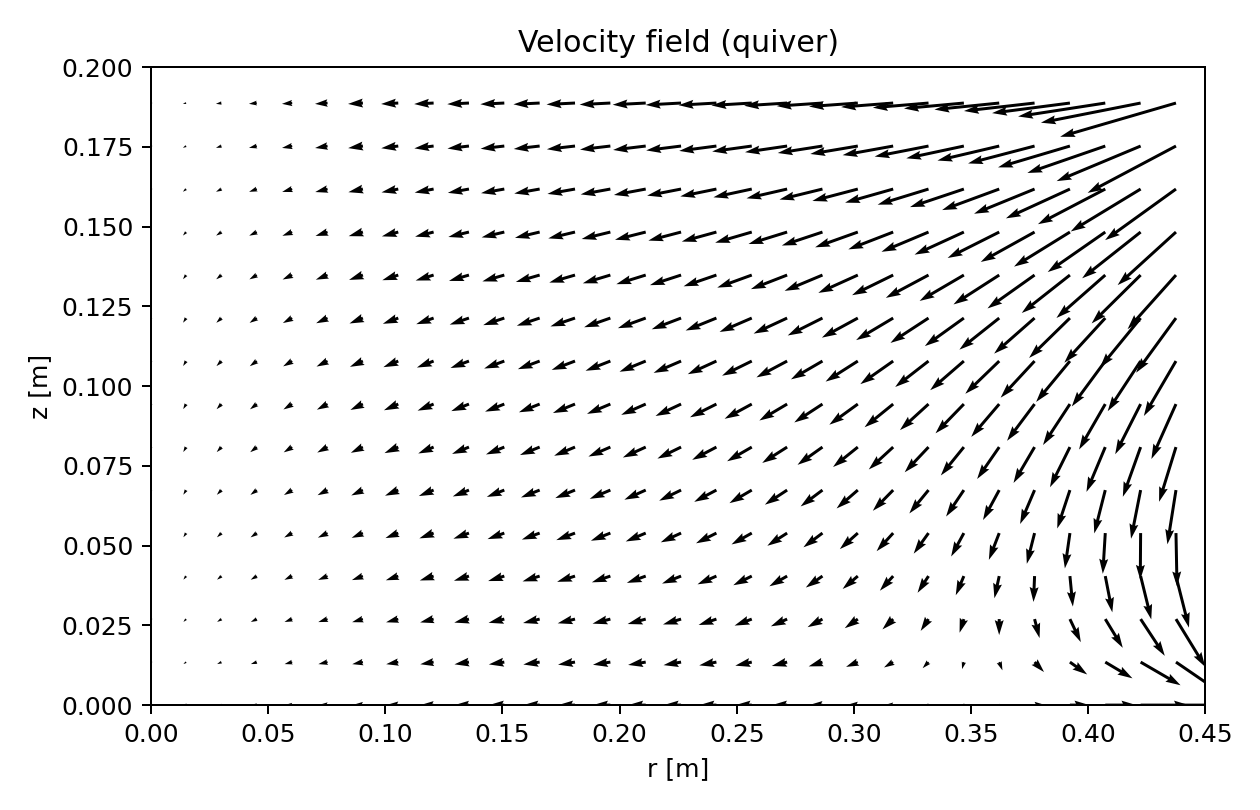
\includegraphics[width=0.95\linewidth]{../figs/quiver_velocity.png}
  \caption{Non-dimensional velocity field (quiver).
Vectors show $(\hat u,\,S\hat w)$ for isotropic visual scaling; the pattern reflects the rim-imposed sealing pressure from the downward curtain.}
  \label{fig:quiver}
\end{figure}\begin{figure}[H]
  \centering
  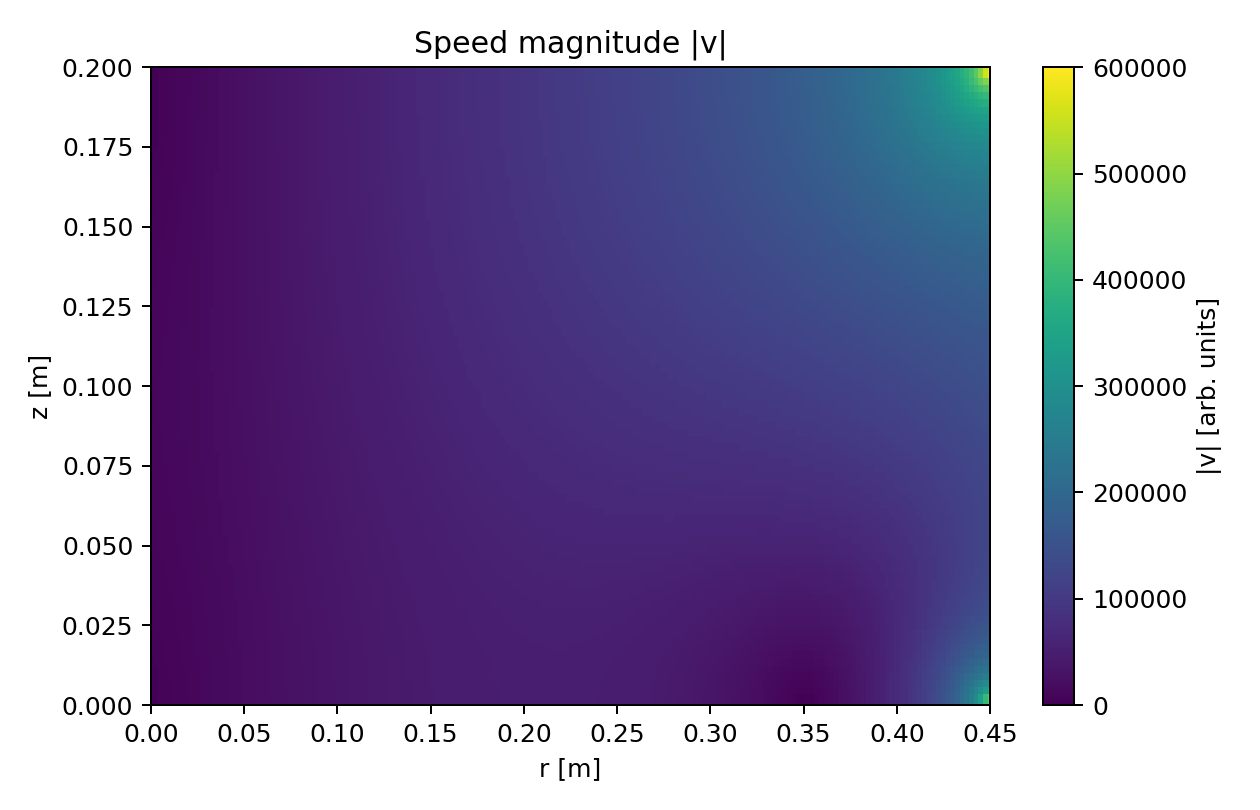
\includegraphics[width=0.95\linewidth]{../figs/cmap_speed.png}
  \caption{Colormap of the non-dimensional isotropic speed magnitude $\hat V_{\mathrm{iso}}=\sqrt{\hat u^{\,2}+S^{2}\hat w^{\,2}}$.}
  \label{fig:cmap_speed}
\end{figure}\begin{figure}[H]
  \centering
  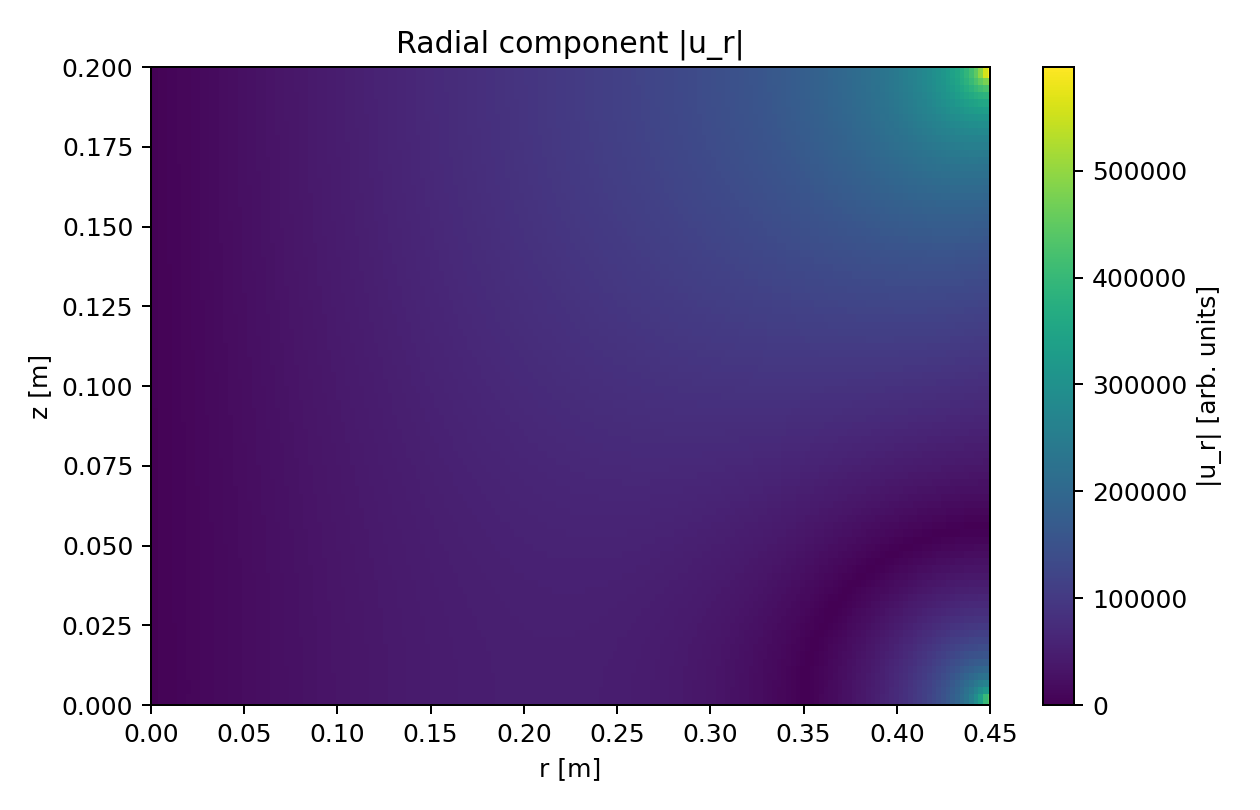
\includegraphics[width=0.95\linewidth]{../figs/cmap_ur.png}
  \caption{Colormap of the non-dimensional radial component magnitude $|\hat u|$.}
  \label{fig:cmap_ur}
\end{figure}\begin{figure}[H]
  \centering
  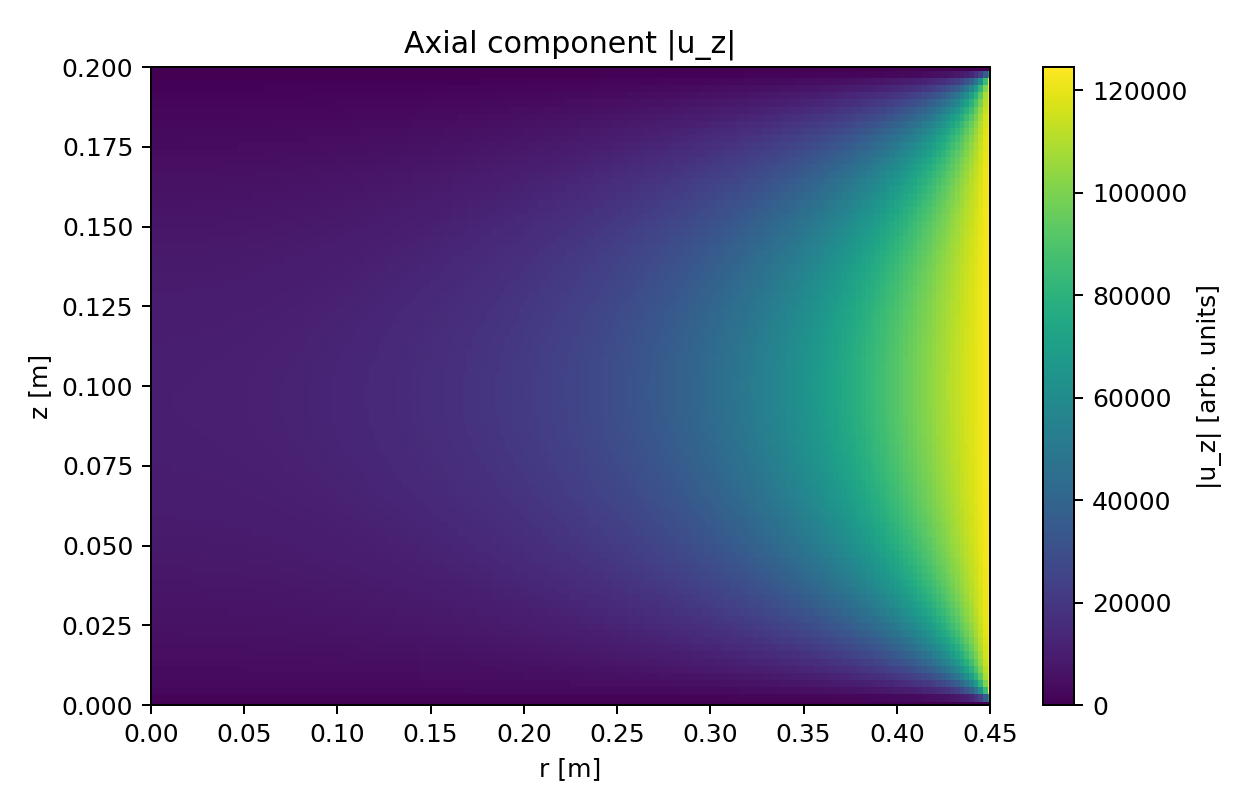
\includegraphics[width=0.95\linewidth]{../figs/cmap_uz.png}
  \caption{Colormap of the non-dimensional axial component magnitude $|\hat w|$.}
  \label{fig:cmap_uz}
\end{figure}\begin{figure}[H]
  \centering
  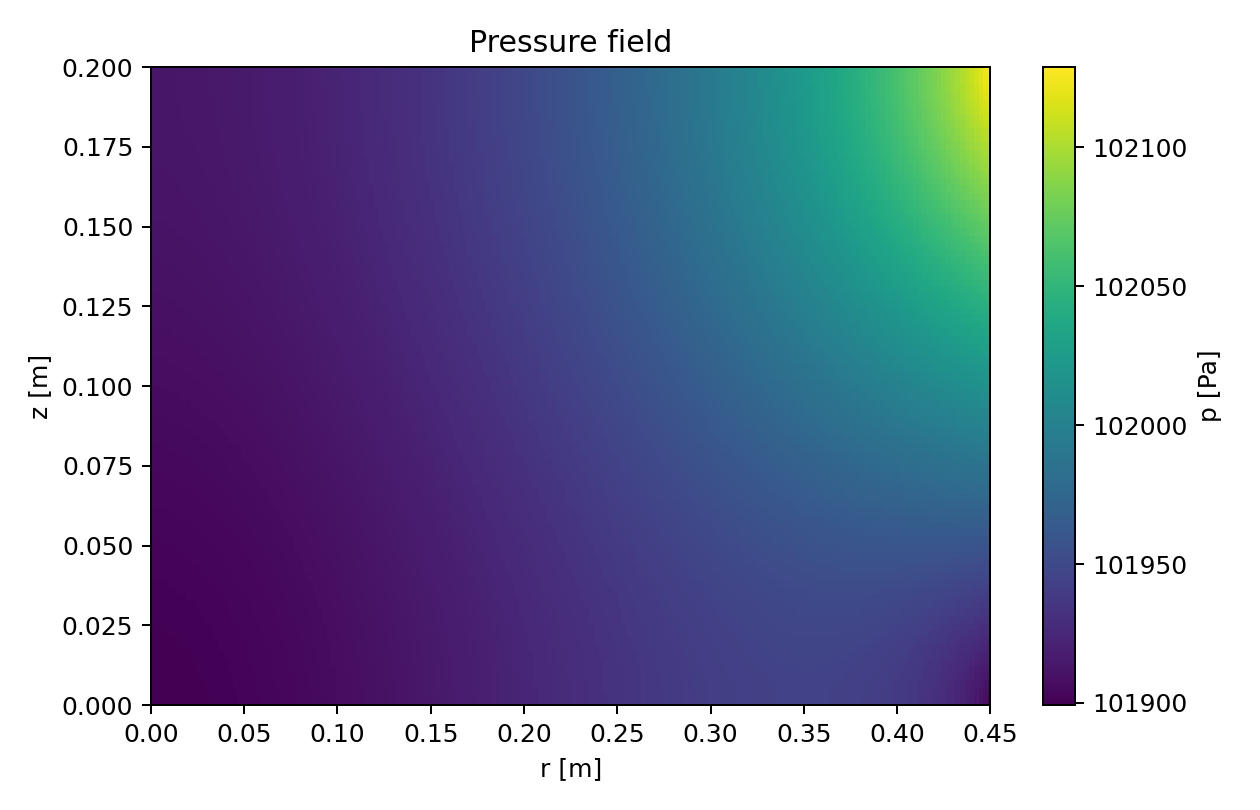
\includegraphics[width=0.95\linewidth]{../figs/cmap_pressure.png}
  \caption{Colormap of the non-dimensional pressure $\hat p$.}
  \label{fig:cmap_p}
\end{figure}

\section{Model Limitations and Planned Extensions}
\label{sec:model-limitations-and-planned-extensions}

The Darcy--Brinkman closure is an engineering reduction (effective permeability in a
free flow); $\alpha_r,\alpha_z$ should be calibrated against axisymmetric CFD.
The make-up jet is not imposed as a local BC in the core; it enters only via the
mass-balance closure. Thermal effects are neglected ($T=T_\infty$). The bypass parameter
$\beta$ is defined conceptually but not used yet in the code; it will be included together
with the automated shooting loop and power estimates.

\paragraph{Appendix: minimal rationale for the composite rim pressure.}
Consider a control volume hugging the rim over height $h$ and thickness $O(b)$.
A downward slot jet of density $\rho_j$ and speed $U_{\mathrm{out}}$ is deflected
into a radial wall-jet of speed $U_r(z)$ near the floor. A crude momentum balance
suggests a static build-up $\Delta p_{\mathrm{stat}}\sim \rho_j U_{\mathrm{out}}^2
\,\mathcal{O}(1)$ concentrated near $\zeta\!\to\!0$, while the resistance to
cross-flow (sealing) scales with the jet momentum flux impinging near the slot,
$\Delta p_{\mathrm{seal}}\sim \rho_j U_{\mathrm{out}}^2\,\mathcal{O}(1)$ for
$\zeta\!\to\!1$. The composite form
$\rho_j U_{\mathrm{out}}^2\,[\,C_p(1-\zeta)^n + C_s \zeta^m\,]$ is thus a
first-order surrogate capturing both effects with two tunable, dimensionless
coefficients $(C_p,C_s)$ and mild shape exponents $(m,n)$.

\paragraph{On the choice of $D_{m,\min}$.}
We take $D_{m,\min}$ from air-curtain literature (order $10^{-1}$) as a design parameter; in absence of calibration, $D_{m,\min}=0.2$ provides a conservative default.
Sensitivity to this parameter is reported without altering the solver or figures.

\paragraph{On the choice of $D_{m,\min}$.}
We adopt $D_{m,\min}=0.2$ as conservative default, consistent with air-curtain literature (typical range $0.1$--$0.3$). The parameter may be refined by CFD or experimental calibration.


\section{Nomenclature}
\label{sec:nomenclature}

\begin{tabular}{@{}ll@{}}
\toprule
Symbol & Description \\ \midrule
$R_{\mathrm{tot}}$ & Total radius of the disc \\
$R^{-}$ & Inner radius of the leakage ring ($R^{-}=R_{\mathrm{tot}}-w$) \\
$w$ & Width of peripheral leakage region \\
$h$ & Hovering height (disc--ground gap) \\
$h_{\mathrm{eff}}$ & Effective sealing height at rim \\
$b$ & Slot thickness of the curtain jet \\
$U_{\mathrm{out}}$ & Outer jet velocity \\
$\rho_j$ & Density of outer jet \\
$\rho$ & Density in the core region \\
$p,p_0,p_c$ & Local, ambient, and cushion pressures \\
$T,T_\infty$ & Local and ambient temperatures \\
$\mu$ & Dynamic viscosity of air \\
$R_g$ & Specific gas constant of air \\
$W$ & Payload supported by cushion \\
$\kappa_r,\kappa_z$ & Effective permeabilities (radial/axial) \\
$\alpha_r,\alpha_z$ & Dimensionless permeability coefficients \\
$u,w$ & Velocity components (radial, vertical) \\
$\Phi(z)$ & Dimensionless rim-pressure distribution \\
$C_t$ & Curtain transfer coefficient \\
$\Delta p$ & Rim pressure increment \\
$\Pi_{\mathrm{edge}}$ & Dimensionless rim pressure amplitude \\
$\mathcal{A}$ & Permeability anisotropy parameter \\
$\hat r,\hat z,\hat p$ & Dimensionless coordinates and pressure \\
$\hat u,\hat w$ & Dimensionless velocity components \\
$S$ & Velocity anisotropy ratio $S=(\alpha_z/\alpha_r)(R_{\mathrm{tot}}/h)$ \\ $D_m$ & Deflection modulus (momentum index) $\rho U_0^2 b_0/(\Delta P\,H)$ \\
$D_{m,\min}$ & Minimum deflection modulus for sealing \\
$b_0$ & Slot thickness at injection (plane jet width) \\
$H$ & Effective curtain height \\
$s$ & Jet spreading parameter ($\approx0.06$--$0.09$) \\
$\Delta P_{\max}$ & Maximum sustainable pressure difference \\
\bottomrule
$C_p$ & static-pressure coefficient for rim build-up (order $10^{-1}$)\\
$C_s$ & sealing-effectiveness coefficient for high-momentum curtain (order $1$)\\
$m,n$ & shape exponents for sealing and static contributions, respectively\\
\end{tabular}

% =====================================================

% --- Added notation for outer-jet seal model ---
\paragraph{Additional symbols.}
\begin{tabular}{ll}
\(r_t\) & effective turning radius of the outer jet \\
\(U_{\mathrm{out}}\) & injection speed of the outer (vertical) jet \\
\(A_{\mathrm{slot}}\) & outlet area of the outer jet \\
\(K_{\mathrm{turn}}\) & momentum loss coefficient at turning (impingement) \\
\(\delta\), \(\delta_t\), \(\delta_s\) & wall-jet thickness (generic / at \(r_t\) / at \(r_-\)) \\
\(U_c(r)\) & characteristic wall-jet speed \\
\(q(r)\), \(m(r)\) & mass and momentum per unit circumference \\
\(E\) & entrainment coefficient \\
\(C_f\) & wall friction coefficient, \(C_f=C_{f0} Re_\delta^{-1/5}\) \\
\(k_e\) & wall-jet thickness growth rate \\
\(w_s\) & seal strip width, \(w_s=\lambda\,\delta_s\) \\
\(\delta_p\) & effective thickness for pressure work in the seal strip \\
\(\Delta p\) & pressure jump between core and ambient
\end{tabular}


\end{document}